
%% !TEX root = manual.tex

\section{Call Graph Visualization}
\label{sec:tutorials:callgraph}
Generating call graphs requires a special build of \sstmacro.

\begin{ShellCmd}
build> ../configure --prefix=$INSTALL_PATH --enable-graphviz
\end{ShellCmd}
The \inlineshell{--enable-graphviz} flag defines an instrumentation macro throughout the \sstmacro code.
This instrumentation must be \emph{compiled} into \sstmacro.
In the default build, the instrumentation is not added since the instrumentation has a high overhead.
However, \sstmacro only instruments a select group of the most important functions so the overhead should only be 10-50\%.
After installing the instrumented version of \sstmacro, a call graph is collected by adding a simple filename to the parameter file.

\begin{ViFile}
call_graph = <fileroot>
\end{ViFile}
After running, a \inlineshell{<fileroot>.callgrind.out} file should appear in the folder.

To visualize the call graph, you must download KCachegrind: \url{http://kcachegrind.sourceforge.net/html/Download.html}.
KCachegrind is built on the KDE environment, which is simple to build for Linux but can be very tedious for Mac.
The download also includes a QCachegrind subfolder, providing the same functionality built on top of Qt.  
This is highly recommended for Mac users.

\begin{figure}[h]
\centering
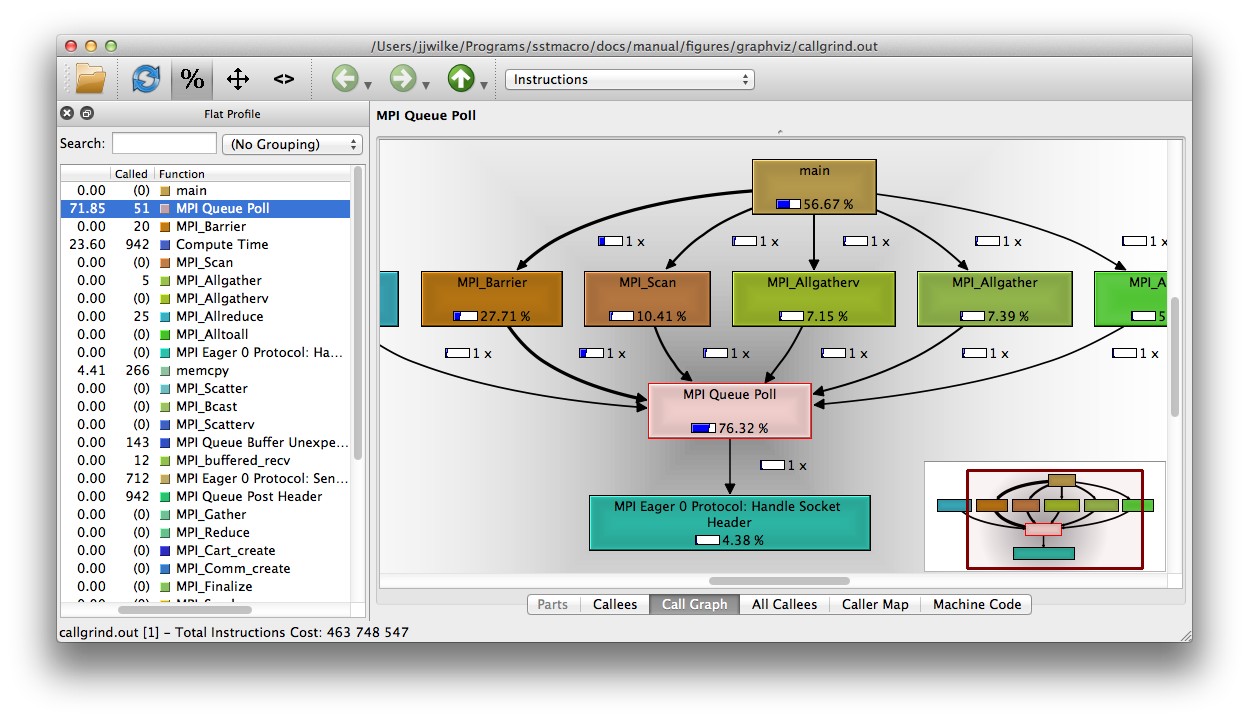
\includegraphics[width=0.95\textwidth]{figures/graphviz/gui.png}
\caption{QCachegrind GUI}
\label{fig:qcgui}
\end{figure}

The basic QCachegrind GUI is shown in Figure \ref{fig:qcgui}.  
On the left, a sidebar contains the list of all functions instrumented with the percent of total execution time spent in the function.
In the center pane, the call graph is shown.  
To navigate the call graph, a small window in the bottom right corner can be used to change the view pane.
Zooming into one region (Figure \ref{fig:qcgraphone}), we see a set of MPI functions (Barrier, Scan, Allgatherv).
Each of the functions enters a polling loop, which dominates the total execution time.  
A small portion of the polling loop calls the ``Handle Socket Header'' function.
Double-clicking this node unrolls more details in the call graph (Figure \ref{fig:qcgraphtwo}).
Here we see the function splits execution time between buffering messages (memcpy) and posting headers (Compute Time).

\begin{figure}[h!]
\centering
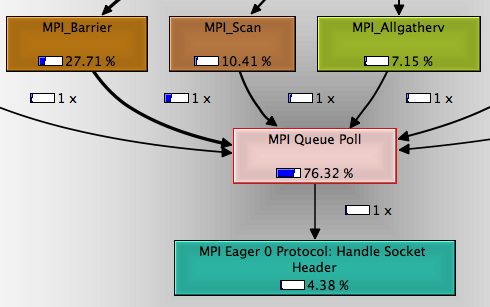
\includegraphics[width=0.55\textwidth]{figures/graphviz/callgraph1.png}
\caption{QCachegrind Call Graph of MPI Functions}
\label{fig:qcgraphone}
\end{figure}

\begin{figure}[h!]
\centering
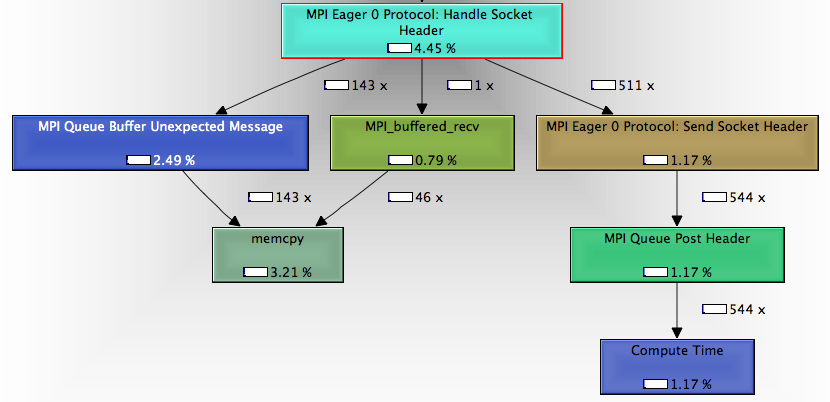
\includegraphics[width=0.75\textwidth]{figures/graphviz/callgraph2.png}
\caption{QCachegrind Expanded Call Graph of Eager 0 Function}
\label{fig:qcgraphtwo}
\end{figure}
